\begin{mdframed}[style=warning]
	\begin{ejercicio}
		\textbf{Conceptos.}
		\begin{enumerate}
			\item Sus manos están húmedas y el dispensador de toallas del baño está vacío. ¿Qué hace para quitar las gotas de agua de sus manos? ¿Cómo su acción ejemplifica una de las leyes de Newton? ¿Cuál de ellas?
			$\mathbf{R//}$ Al sacudir las manos se ve claramente la acción de la inercia, haciendo que las gotas sigan el movimiento dado al momento de cambiar de dirección la mano. Primera Ley de Newton.
			\item ¿Un objeto puede ejercer una fuerza sobre sí mismo? Argumente. $\mathbf{R//}$ No, por la tercera Ley de Newton.
			\item Una cubeta de agua se puede girar en una trayectoria vertical tal que no se derrame agua. ¿Por qué el agua permanece en la cubeta, aun cuando la cubeta esté sobre su cabeza? $\mathbf{R//}$ Gracias a la primera ley de Newton, la acción de la fuerza centrífuga (la cual es una fuerza ficticia), hace que el agua quiera seguir su estado de movimiento y por ende, mantenerse en la cubeta.
			\item ¿Por qué un piloto tiende a desmayarse cuando sale de una pronunciada caída en picada? $\mathbf{R//}$ La idea es la misma que el inciso anterior, la presión sanguínea no es suficiente para vencer a la inercia y el aumento relativo del peso, por lo que no llega suficiente sangre al cerebro. Esto causa los desmayos e incluso, si ocurre por un lapso muy prolongado de tiempo, la muerte.
		\end{enumerate}
	\end{ejercicio}
\end{mdframed}





\begin{mdframed}[style=warning]
	\begin{ejercicio}
		El bloque $A$, de peso $3w$, se desliza con rapidez constante, bajando por un plano $S$ inclinado $36.9^o$, mientras la tabla $B$, de peso $w$, descansa sobre $A$, estando sujeta con una cuerda a la pared. Si el coeficiente de fricción es igual entre $A$ y $B$ y entre $S$ y $A$, determine su valor.
		\begin{figure}[H]
			\centering
			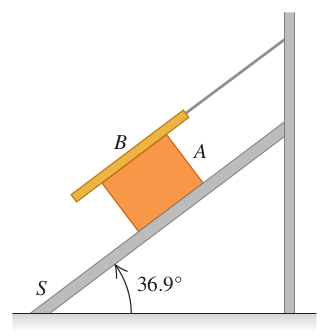
\includegraphics[scale=0.35]{./img/599.png}
			\caption{Ejercicio 2}
			\label{599}
		\end{figure}
	\end{ejercicio}
	\noindent \textbf{Solución: } \\
	Para este problema se tienen los siguientes diagramas de cuerpo libre y sus respectivas sumatorias de fuerzas en ambos ejes (con el sistema de referencia rotado de modo que el eje $x$ sea paralelo al plano).
	\begin{multicols}{2}
		


\tikzset{every picture/.style={line width=0.75pt}} %set default line width to 0.75pt        

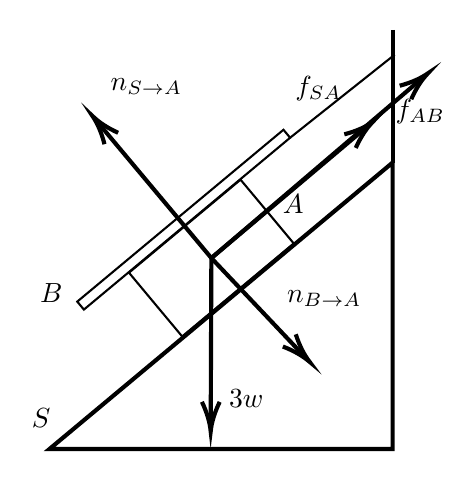
\begin{tikzpicture}[x=0.75pt,y=0.75pt,yscale=-1,xscale=1]
%uncomment if require: \path (0,300); %set diagram left start at 0, and has height of 300

%Shape: Right Triangle [id:dp05774627415960376] 
\draw  [line width=1.5]  (413.33,108) -- (248,246) -- (413.33,246) -- cycle ;
%Straight Lines [id:da4295758086182351] 
\draw [line width=1.5]    (413.33,44) -- (413.33,108) ;
%Shape: Rectangle [id:dp3252104103742237] 
\draw   (286.31,161.05) -- (340.07,116.23) -- (365.69,146.95) -- (311.93,191.77) -- cycle ;
%Shape: Rectangle [id:dp3516245066512129] 
\draw   (261.39,174.98) -- (360.74,92.18) -- (363.94,96.02) -- (264.59,178.82) -- cycle ;
%Straight Lines [id:da5643038396039826] 
\draw    (363.94,96.02) -- (414.33,56) ;
%Straight Lines [id:da4964837166601317] 
\draw [line width=1.5]    (326,154) -- (325.68,234.5) ;
\draw [shift={(325.67,237.5)}, rotate = 270.23] [color={rgb, 255:red, 0; green, 0; blue, 0 }  ][line width=1.5]    (14.21,-4.28) .. controls (9.04,-1.82) and (4.3,-0.39) .. (0,0) .. controls (4.3,0.39) and (9.04,1.82) .. (14.21,4.28)   ;
%Straight Lines [id:da28582174108367076] 
\draw [line width=1.5]    (326,154) -- (428.05,66.95) ;
\draw [shift={(430.33,65)}, rotate = 139.53] [color={rgb, 255:red, 0; green, 0; blue, 0 }  ][line width=1.5]    (14.21,-4.28) .. controls (9.04,-1.82) and (4.3,-0.39) .. (0,0) .. controls (4.3,0.39) and (9.04,1.82) .. (14.21,4.28)   ;
%Straight Lines [id:da8561679038847163] 
\draw [line width=1.5]    (326,154) -- (401.37,90.43) ;
\draw [shift={(403.67,88.5)}, rotate = 139.86] [color={rgb, 255:red, 0; green, 0; blue, 0 }  ][line width=1.5]    (14.21,-4.28) .. controls (9.04,-1.82) and (4.3,-0.39) .. (0,0) .. controls (4.3,0.39) and (9.04,1.82) .. (14.21,4.28)   ;
%Straight Lines [id:da9305052430717813] 
\draw [line width=1.5]    (326,154) -- (270.59,87.8) ;
\draw [shift={(268.67,85.5)}, rotate = 50.07] [color={rgb, 255:red, 0; green, 0; blue, 0 }  ][line width=1.5]    (14.21,-4.28) .. controls (9.04,-1.82) and (4.3,-0.39) .. (0,0) .. controls (4.3,0.39) and (9.04,1.82) .. (14.21,4.28)   ;
%Straight Lines [id:da3352183924103149] 
\draw [line width=1.5]    (326,154) -- (371.27,201.82) ;
\draw [shift={(373.33,204)}, rotate = 226.57] [color={rgb, 255:red, 0; green, 0; blue, 0 }  ][line width=1.5]    (14.21,-4.28) .. controls (9.04,-1.82) and (4.3,-0.39) .. (0,0) .. controls (4.3,0.39) and (9.04,1.82) .. (14.21,4.28)   ;

% Text Node
\draw (242,165) node [anchor=north west][inner sep=0.75pt]    {$B$};
% Text Node
\draw (359,122) node [anchor=north west][inner sep=0.75pt]    {$A$};
% Text Node
\draw (238,225) node [anchor=north west][inner sep=0.75pt]    {$S$};
% Text Node
\draw (361,168) node [anchor=north west][inner sep=0.75pt]    {$n_{B\rightarrow A}$};
% Text Node
\draw (333,216) node [anchor=north west][inner sep=0.75pt]    {$3w$};
% Text Node
\draw (276,66) node [anchor=north west][inner sep=0.75pt]    {$n_{S\rightarrow A}$};
% Text Node
\draw (365,65) node [anchor=north west][inner sep=0.75pt]    {$f_{SA}$};
% Text Node
\draw (413.33,76) node [anchor=north west][inner sep=0.75pt]    {$f_{AB}$};


\end{tikzpicture}

		\begin{align*}
			\sum F_x &= 0 \\
			3w\sin{\theta} &= f_{AB} + f_{SA} \numberthis \label{ej2_dclA_x} \\
			\sum F_y &= 0 \\
			n_{SA} &= n_{BA} + 3w\cos{\theta} \numberthis \label{ej2_dclA_y}
		\end{align*}
		\columnbreak
		


\tikzset{every picture/.style={line width=0.75pt}} %set default line width to 0.75pt        

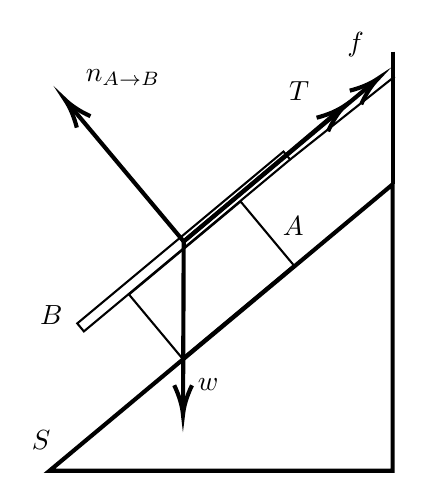
\begin{tikzpicture}[x=0.75pt,y=0.75pt,yscale=-1,xscale=1]
%uncomment if require: \path (0,300); %set diagram left start at 0, and has height of 300

%Shape: Right Triangle [id:dp05774627415960376] 
\draw  [line width=1.5]  (413.33,108) -- (248,246) -- (413.33,246) -- cycle ;
%Straight Lines [id:da4295758086182351] 
\draw [line width=1.5]    (413.33,44) -- (413.33,108) ;
%Shape: Rectangle [id:dp3252104103742237] 
\draw   (286.31,161.05) -- (340.07,116.23) -- (365.69,146.95) -- (311.93,191.77) -- cycle ;
%Shape: Rectangle [id:dp3516245066512129] 
\draw   (261.39,174.98) -- (360.74,92.18) -- (363.94,96.02) -- (264.59,178.82) -- cycle ;
%Straight Lines [id:da5643038396039826] 
\draw    (363.94,96.02) -- (414.33,56) ;
%Straight Lines [id:da4964837166601317] 
\draw [line width=1.5]    (312.67,135.5) -- (312.35,216) ;
\draw [shift={(312.33,219)}, rotate = 270.23] [color={rgb, 255:red, 0; green, 0; blue, 0 }  ][line width=1.5]    (14.21,-4.28) .. controls (9.04,-1.82) and (4.3,-0.39) .. (0,0) .. controls (4.3,0.39) and (9.04,1.82) .. (14.21,4.28)   ;
%Straight Lines [id:da28582174108367076] 
\draw [line width=1.5]    (312.67,135.5) -- (404.03,58.93) ;
\draw [shift={(406.33,57)}, rotate = 140.03] [color={rgb, 255:red, 0; green, 0; blue, 0 }  ][line width=1.5]    (14.21,-4.28) .. controls (9.04,-1.82) and (4.3,-0.39) .. (0,0) .. controls (4.3,0.39) and (9.04,1.82) .. (14.21,4.28)   ;
%Straight Lines [id:da8561679038847163] 
\draw [line width=1.5]    (312.67,135.5) -- (388.04,71.93) ;
\draw [shift={(390.33,70)}, rotate = 139.86] [color={rgb, 255:red, 0; green, 0; blue, 0 }  ][line width=1.5]    (14.21,-4.28) .. controls (9.04,-1.82) and (4.3,-0.39) .. (0,0) .. controls (4.3,0.39) and (9.04,1.82) .. (14.21,4.28)   ;
%Straight Lines [id:da9305052430717813] 
\draw [line width=1.5]    (312.67,135.5) -- (257.26,69.3) ;
\draw [shift={(255.33,67)}, rotate = 50.07] [color={rgb, 255:red, 0; green, 0; blue, 0 }  ][line width=1.5]    (14.21,-4.28) .. controls (9.04,-1.82) and (4.3,-0.39) .. (0,0) .. controls (4.3,0.39) and (9.04,1.82) .. (14.21,4.28)   ;

% Text Node
\draw (242,165) node [anchor=north west][inner sep=0.75pt]    {$B$};
% Text Node
\draw (359,122) node [anchor=north west][inner sep=0.75pt]    {$A$};
% Text Node
\draw (238,225) node [anchor=north west][inner sep=0.75pt]    {$S$};
% Text Node
\draw (264,51) node [anchor=north west][inner sep=0.75pt]    {$n_{A\rightarrow B}$};
% Text Node
\draw (318,200) node [anchor=north west][inner sep=0.75pt]    {$w$};
% Text Node
\draw (390,33) node [anchor=north west][inner sep=0.75pt]    {$f$};
% Text Node
\draw (362,57) node [anchor=north west][inner sep=0.75pt]    {$T$};


\end{tikzpicture}

		Para el bloque $B$ no nos interesa el eje $x$.
		\begin{align*}
			\sum F_y &= 0 \\
			n_{AB} &= w\cos{\theta} \numberthis \label{ej2_dclB_y}
		\end{align*}
	\end{multicols}
	Además, por tercera ley de Newton, sabemos que $\abs{n_{AB}} = \abs{n_{BA}}$ y por definición $f_{AB} = \mu n_{AB}$ y $f_{SA} = \mu n_{SA}$. Con esto, resolvemos el sistema de ecuaciones y se tiene
		$$ 3w\sin{\theta} = 5w\mu \cos{\theta}, $$
		$$ \therefore \quad \boxed{ \mu = \frac{3}{5} \tan{\theta} = 0.45 } $$
\end{mdframed}







\begin{mdframed}[style=warning]
	\begin{ejercicio}
		Una cuenta pequeña puede desliarse sin fricción por un aro circular de $0.1m$ de radio, que está e un plano vertical. El aro gira con velocidad constante de $4rev/s$ en torno a un diametro vertical. \textit{(a)} Calcule el ángulo $\beta$ en el que la cuenta está en equilibrio vertical. \textit{(b)} ¿La cuenta podría permanecer a la misma altura que el centro del aro?
		\begin{figure}[H]
			\centering
			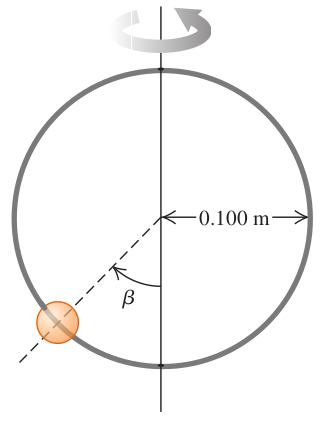
\includegraphics[scale=0.35]{./img/5119.png}
			\caption{Ejercicio 3}
			\label{5119}
		\end{figure}
	\end{ejercicio}
	\noindent \textbf{Solución: } \\
	\textit{(a)} En el momento de equilibrio vertical se tiene el siguiente diagrama de cuerpo libre:
	\begin{center}
		


\tikzset{every picture/.style={line width=0.75pt}} %set default line width to 0.75pt        

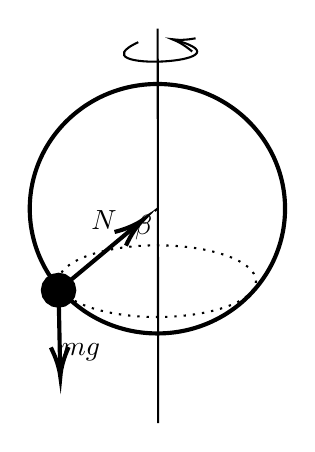
\begin{tikzpicture}[x=0.75pt,y=0.75pt,yscale=-1,xscale=1]
%uncomment if require: \path (0,300); %set diagram left start at 0, and has height of 300

%Shape: Ellipse [id:dp7235707808939753] 
\draw  [line width=1.5]  (268.33,133.72) .. controls (268.33,100.53) and (295.87,73.63) .. (329.83,73.63) .. controls (363.8,73.63) and (391.33,100.53) .. (391.33,133.72) .. controls (391.33,166.91) and (363.8,193.82) .. (329.83,193.82) .. controls (295.87,193.82) and (268.33,166.91) .. (268.33,133.72) -- cycle ;
%Shape: Ellipse [id:dp5004444881185273] 
\draw  [dash pattern={on 0.84pt off 2.51pt}] (282.2,168.63) .. controls (282.2,159.09) and (303.5,151.36) .. (329.77,151.36) .. controls (356.04,151.36) and (377.34,159.09) .. (377.34,168.63) .. controls (377.34,178.17) and (356.04,185.9) .. (329.77,185.9) .. controls (303.5,185.9) and (282.2,178.17) .. (282.2,168.63) -- cycle ;
%Straight Lines [id:da8772179839412539] 
\draw    (329.96,47) -- (330.2,237) ;
%Shape: Ellipse [id:dp23606665212662592] 
\draw  [fill={rgb, 255:red, 0; green, 0; blue, 0 }  ,fill opacity=1 ][line width=6]  (277.72,173.01) .. controls (277.72,170.59) and (279.73,168.63) .. (282.2,168.63) .. controls (284.68,168.63) and (286.69,170.59) .. (286.69,173.01) .. controls (286.69,175.42) and (284.68,177.39) .. (282.2,177.39) .. controls (279.73,177.39) and (277.72,175.42) .. (277.72,173.01) -- cycle ;
%Straight Lines [id:da6990477011010658] 
\draw  [dash pattern={on 4.5pt off 4.5pt}]  (282.2,173.01) -- (329.83,133.72) ;
%Curve Lines [id:da35614337048743017] 
\draw    (320.63,53.48) .. controls (288.71,68.36) and (378.27,63.7) .. (338.73,52.55) ;
\draw [shift={(336.83,52.04)}, rotate = 14.6] [color={rgb, 255:red, 0; green, 0; blue, 0 }  ][line width=0.75]    (10.93,-3.29) .. controls (6.95,-1.4) and (3.31,-0.3) .. (0,0) .. controls (3.31,0.3) and (6.95,1.4) .. (10.93,3.29)   ;
%Straight Lines [id:da3142740996221758] 
\draw [line width=1.5]    (282.2,173.01) -- (320.53,141.04) ;
\draw [shift={(322.84,139.12)}, rotate = 140.17] [color={rgb, 255:red, 0; green, 0; blue, 0 }  ][line width=1.5]    (14.21,-4.28) .. controls (9.04,-1.82) and (4.3,-0.39) .. (0,0) .. controls (4.3,0.39) and (9.04,1.82) .. (14.21,4.28)   ;
%Straight Lines [id:da26678286412782426] 
\draw [line width=1.5]    (282.2,173.01) -- (283,211.69) ;
\draw [shift={(283.06,214.69)}, rotate = 268.82] [color={rgb, 255:red, 0; green, 0; blue, 0 }  ][line width=1.5]    (14.21,-4.28) .. controls (9.04,-1.82) and (4.3,-0.39) .. (0,0) .. controls (4.3,0.39) and (9.04,1.82) .. (14.21,4.28)   ;

% Text Node
\draw (317.54,135.32) node [anchor=north west][inner sep=0.75pt]    {$\beta $};
% Text Node
\draw (282.21,197.21) node [anchor=north west][inner sep=0.75pt]    {$mg$};
% Text Node
\draw (296.52,133.16) node [anchor=north west][inner sep=0.75pt]    {$N$};


\end{tikzpicture}
	
	\end{center}
	Con esto, se tienen las siguientes sumatorias de fuerza, entendiendo que la línea punteada es la trayectoria que sigue la cuenta
	\begin{align*}
		\sum F_x &= ma_c \\
		N\sin{\beta} &= ma_c = 4\pi ^2 \nu ^2 mR\sin{\beta} \numberthis \label{ej3_dcl_x} \\
		\sum F_y &= 0 \quad \text{(equilibrio vertical)} \\
		N\cos{\beta} &= mg. \numberthis \label{ej3_dcl_y}
	\end{align*}
	Dividiendo \eqref{ej3_dcl_x} entre \eqref{ej3_dcl_y} y despejando el ángulo, se tiene
		$$ \boxed{ \beta = \cos ^{-1} {\qty(\frac{g}{4\pi ^2 \nu ^2 R})} = 81.1^o . } $$
	\textit{(b)} No, ya que si la cuenta está a la altura del centro del aro, se tiene $\beta \to \frac{\pi}{2}$ lo que implica una frecuencia $\nu \to \infty$, cosa que es imposible.
\end{mdframed}

















\begin{mdframed}[style=warning]
	\begin{ejercicio}
		Si un bloque cuadrado se desliza por una cuña con ángulo recto inclinada un ángulo $\theta$. El coeficiente de fricción cinético entre la cuña y el bloque es $\mu _k$. ¿Cuál es la aceleración del bloque en términos de las variables conocidas?
		\begin{figure}[H]
			\centering
			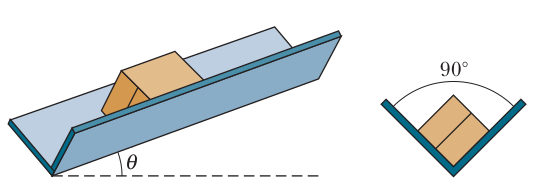
\includegraphics[scale=0.3]{./img/cuna.png}
			\caption{Ejercicio 4}
		\end{figure}
	\end{ejercicio}
	\noindent \textbf{Solución: } \\
	Realizamos los diagramas de cuerpo libre.
	\begin{center}
		


\tikzset{every picture/.style={line width=0.75pt}} %set default line width to 0.75pt        

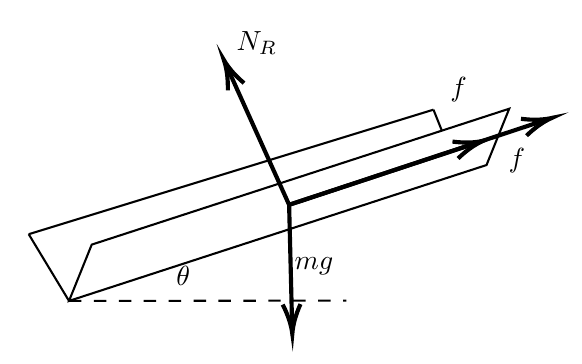
\begin{tikzpicture}[x=0.75pt,y=0.75pt,yscale=-1,xscale=1]
%uncomment if require: \path (0,307); %set diagram left start at 0, and has height of 307

%Shape: Parallelogram [id:dp1789874265842366] 
\draw   (231.69,157.02) -- (432.83,91.55) -- (421.9,118.68) -- (220.75,184.15) -- cycle ;
%Straight Lines [id:da8186159047615356] 
\draw    (220.75,184.15) -- (201.33,152) ;
%Straight Lines [id:da21449158239762323] 
\draw    (201.33,152) -- (396.33,92) ;
%Straight Lines [id:da4125441507452967] 
\draw    (396.33,92) -- (400.33,102) ;
%Straight Lines [id:da05828595981571327] 
\draw [line width=1.5]    (326.79,137.85) -- (328.26,197) ;
\draw [shift={(328.33,200)}, rotate = 268.58] [color={rgb, 255:red, 0; green, 0; blue, 0 }  ][line width=1.5]    (14.21,-4.28) .. controls (9.04,-1.82) and (4.3,-0.39) .. (0,0) .. controls (4.3,0.39) and (9.04,1.82) .. (14.21,4.28)   ;
%Straight Lines [id:da3030463052785377] 
\draw [line width=1.5]    (326.79,137.85) -- (296.57,70.74) ;
\draw [shift={(295.33,68)}, rotate = 65.75] [color={rgb, 255:red, 0; green, 0; blue, 0 }  ][line width=1.5]    (14.21,-4.28) .. controls (9.04,-1.82) and (4.3,-0.39) .. (0,0) .. controls (4.3,0.39) and (9.04,1.82) .. (14.21,4.28)   ;
%Straight Lines [id:da16864728132898277] 
\draw [line width=1.5]    (326.79,137.85) -- (450.49,96.94) ;
\draw [shift={(453.33,96)}, rotate = 161.7] [color={rgb, 255:red, 0; green, 0; blue, 0 }  ][line width=1.5]    (14.21,-4.28) .. controls (9.04,-1.82) and (4.3,-0.39) .. (0,0) .. controls (4.3,0.39) and (9.04,1.82) .. (14.21,4.28)   ;
%Straight Lines [id:da49421953060492485] 
\draw [line width=1.5]    (326.79,137.85) -- (417.48,107.94) ;
\draw [shift={(420.33,107)}, rotate = 161.75] [color={rgb, 255:red, 0; green, 0; blue, 0 }  ][line width=1.5]    (14.21,-4.28) .. controls (9.04,-1.82) and (4.3,-0.39) .. (0,0) .. controls (4.3,0.39) and (9.04,1.82) .. (14.21,4.28)   ;
%Straight Lines [id:da46233372838154385] 
\draw  [dash pattern={on 4.5pt off 4.5pt}]  (220.75,184.15) -- (354.33,184) ;

% Text Node
\draw (271,166) node [anchor=north west][inner sep=0.75pt]    {$\theta $};
% Text Node
\draw (328,162) node [anchor=north west][inner sep=0.75pt]    {$mg$};
% Text Node
\draw (300,53) node [anchor=north west][inner sep=0.75pt]    {$N_{R}$};
% Text Node
\draw (403,75) node [anchor=north west][inner sep=0.75pt]    {$f$};
% Text Node
\draw (431,109) node [anchor=north west][inner sep=0.75pt]    {$f$};


\end{tikzpicture}

		\vspace{0.5cm}
		


\tikzset{every picture/.style={line width=0.75pt}} %set default line width to 0.75pt        

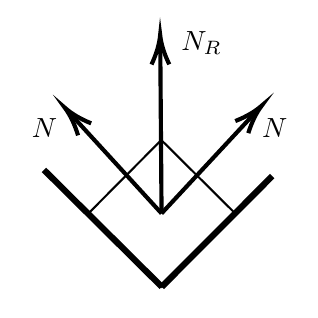
\begin{tikzpicture}[x=0.75pt,y=0.75pt,yscale=-1,xscale=1]
%uncomment if require: \path (0,307); %set diagram left start at 0, and has height of 307

%Shape: Square [id:dp11158416935531834] 
\draw   (293.64,158.12) -- (328.88,122.64) -- (364.36,157.88) -- (329.12,193.36) -- cycle ;
%Straight Lines [id:da5782322433552698] 
\draw [line width=2.25]    (272.33,137) -- (329.12,193.36) ;
%Straight Lines [id:da31004030039107744] 
\draw [line width=2.25]    (329.12,193.36) -- (382.33,140) ;
%Straight Lines [id:da7515473055819413] 
\draw [line width=1.5]    (329,158) -- (375.29,108.2) ;
\draw [shift={(377.33,106)}, rotate = 132.91] [color={rgb, 255:red, 0; green, 0; blue, 0 }  ][line width=1.5]    (14.21,-4.28) .. controls (9.04,-1.82) and (4.3,-0.39) .. (0,0) .. controls (4.3,0.39) and (9.04,1.82) .. (14.21,4.28)   ;
%Straight Lines [id:da17146564901097117] 
\draw [line width=1.5]    (329,158) -- (284.36,109.21) ;
\draw [shift={(282.33,107)}, rotate = 47.54] [color={rgb, 255:red, 0; green, 0; blue, 0 }  ][line width=1.5]    (14.21,-4.28) .. controls (9.04,-1.82) and (4.3,-0.39) .. (0,0) .. controls (4.3,0.39) and (9.04,1.82) .. (14.21,4.28)   ;
%Straight Lines [id:da34529906812085653] 
\draw [line width=1.5]    (329,158) -- (328.36,75) ;
\draw [shift={(328.33,72)}, rotate = 89.56] [color={rgb, 255:red, 0; green, 0; blue, 0 }  ][line width=1.5]    (14.21,-4.28) .. controls (9.04,-1.82) and (4.3,-0.39) .. (0,0) .. controls (4.3,0.39) and (9.04,1.82) .. (14.21,4.28)   ;

% Text Node
\draw (265,111) node [anchor=north west][inner sep=0.75pt]    {$N$};
% Text Node
\draw (376,111) node [anchor=north west][inner sep=0.75pt]    {$N$};
% Text Node
\draw (337,69) node [anchor=north west][inner sep=0.75pt]    {$N_{R}$};


\end{tikzpicture}

	\end{center}
	Como se ve en el segundo diagrama, la fuerza normal resultante es la suma vectorial de las dos fuerzas normales presentes, una por cada superficie de contacto, $N_R = \sqrt{2} N$. Ahora, tomando el primer diagrama, realizamos la sumatoria de fuerzas (con el sistema de referencia rotado)
		\begin{align*}
			\sum F_x &= ma \\
			ma &= mg\sin{\theta} - 2f \numberthis \label{ej4_dcl_x} \\
			\sum F_y &= 0 \\
			N_R &= mg\cos{\theta}. \numberthis \label{ej4_dcl_y}
		\end{align*}
	Resolviendo el sistema de ecuaciones sabiendo que $f = \mu _k N$ (ojo, aquí la fuerza normal relacionada con la fricción es la presente en cada superficie, no la resultante.)
		$$ \boxed{ a = g\qty(\sin{\theta} - \sqrt{2} \mu _k \cos{\theta}). } $$
\end{mdframed}








\begin{mdframed}[style=warning]
	\begin{ejercicio}
		Un bloque pequeño de masa $m$ se coloca dentro de un cono invertido que gira sobre un eje vertical, de modo que la duración de una revolución del cono es $T$. La pared del cono forma un ángulo $\beta$ con la horizontal. El coeficiente de fricción estática entre el bloque y el cono es $\mu _s$. Si el bloque debe mantenerse a una altura constante $h$ sobre el vértice del cono. ¿Cuáles son el valor máximo y mínimo de $T$?
	\end{ejercicio}
	\noindent \textbf{Solución: } \\
	Primero, es necesario saber que pasa con el bloque para cada uno de los casos. Para el caso del periodo máximo, se tiene un tiempo por fuelta muy alto, por ende una frecuencia muy baja, el bloque tiende a deslizarse hacia abajo. Con esto, el diagrama de cuerpo libre del bloque sería:
		\begin{center}
			


\tikzset{every picture/.style={line width=0.75pt}} %set default line width to 0.75pt        

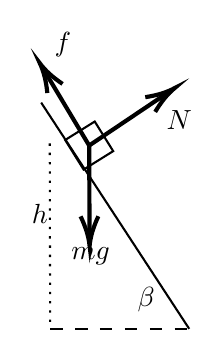
\begin{tikzpicture}[x=0.75pt,y=0.75pt,yscale=-1,xscale=1]
%uncomment if require: \path (0,307); %set diagram left start at 0, and has height of 307

%Straight Lines [id:da2346043214601068] 
\draw    (295,123) -- (366.33,232) ;
%Straight Lines [id:da8690308221217631] 
\draw  [dash pattern={on 4.5pt off 4.5pt}]  (299.33,232) -- (366.33,232) ;
%Shape: Square [id:dp4393211395057455] 
\draw   (320.81,132.12) -- (329.7,146.38) -- (315.45,155.26) -- (306.56,141.01) -- cycle ;
%Straight Lines [id:da9111945804366643] 
\draw  [dash pattern={on 0.84pt off 2.51pt}]  (299.13,142.69) -- (299.33,232) ;
%Straight Lines [id:da11668429195135088] 
\draw [line width=1.5]    (318.13,143.69) -- (318.32,189) ;
\draw [shift={(318.33,192)}, rotate = 269.76] [color={rgb, 255:red, 0; green, 0; blue, 0 }  ][line width=1.5]    (14.21,-4.28) .. controls (9.04,-1.82) and (4.3,-0.39) .. (0,0) .. controls (4.3,0.39) and (9.04,1.82) .. (14.21,4.28)   ;
%Straight Lines [id:da8514966458719733] 
\draw [line width=1.5]    (318.13,143.69) -- (356.84,117.67) ;
\draw [shift={(359.33,116)}, rotate = 146.09] [color={rgb, 255:red, 0; green, 0; blue, 0 }  ][line width=1.5]    (14.21,-4.28) .. controls (9.04,-1.82) and (4.3,-0.39) .. (0,0) .. controls (4.3,0.39) and (9.04,1.82) .. (14.21,4.28)   ;
%Straight Lines [id:da7352305231215699] 
\draw [line width=1.5]    (318.13,143.69) -- (295.88,106.57) ;
\draw [shift={(294.33,104)}, rotate = 59.06] [color={rgb, 255:red, 0; green, 0; blue, 0 }  ][line width=1.5]    (14.21,-4.28) .. controls (9.04,-1.82) and (4.3,-0.39) .. (0,0) .. controls (4.3,0.39) and (9.04,1.82) .. (14.21,4.28)   ;

% Text Node
\draw (340,210.4) node [anchor=north west][inner sep=0.75pt]    {$\beta $};
% Text Node
\draw (289,170.4) node [anchor=north west][inner sep=0.75pt]    {$h$};
% Text Node
\draw (300,87.4) node [anchor=north west][inner sep=0.75pt]    {$f$};
% Text Node
\draw (354,125.4) node [anchor=north west][inner sep=0.75pt]    {$N$};
% Text Node
\draw (308,191.4) node [anchor=north west][inner sep=0.75pt]    {$mg$};


\end{tikzpicture}

		\end{center}
	Con esto, solo es necesario realizar un poco de geometría para encontrar cada uno de los ángulos (tanto para la normal, como para la fricción) y realizamos la sumatoria de fuerzas para cada uno de los ejes (ojo que no rotamos el plano, la aceleració centrípeta va en dirección horizontal hacia el eje del cono). Reemplazando directamente $f = \mu N$.
	\begin{align*}
		\sum F_x &= ma_c \\
		m\frac{4\pi ^2 h}{T_{\text{MAX}} ^2 \tan{\beta}} &= N\sen{\beta} - \mu N \cos{\beta} \numberthis \label{ej5_dcl1_x} \\
		\sum F_y &= 0 \\
		mg &= N\cos{\beta} + \mu \sin{\beta}. \numberthis \label{ej5_dcl1_y}
	\end{align*}
	Se divide \eqref{ej5_dcl1_y} entre \eqref{ej5_dcl1_x} y se despeja el periodo
		$$ \boxed{ T_{\text{MAX}} = 2\pi \sqrt{\frac{h}{g\tan{\beta}} \frac{\cos{\beta} + \mu \sin{\beta}}{\sin{\beta} - \mu \cos{\beta}} } . } $$
		
	Ahora, para el periodo mínimo se tiene lo opuesto, la frecuencia es alta y el bloque tiende a salir del cono, por lo que el diagrama de cuerpo libre sería:
	\begin{center}
		


\tikzset{every picture/.style={line width=0.75pt}} %set default line width to 0.75pt        

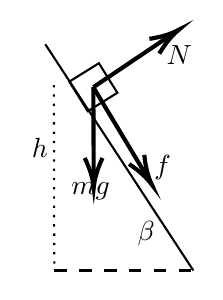
\begin{tikzpicture}[x=0.75pt,y=0.75pt,yscale=-1,xscale=1]
%uncomment if require: \path (0,307); %set diagram left start at 0, and has height of 307

%Straight Lines [id:da2346043214601068] 
\draw    (295,123) -- (366.33,232) ;
%Straight Lines [id:da8690308221217631] 
\draw  [dash pattern={on 4.5pt off 4.5pt}]  (299.33,232) -- (366.33,232) ;
%Shape: Square [id:dp4393211395057455] 
\draw   (320.81,132.12) -- (329.7,146.38) -- (315.45,155.26) -- (306.56,141.01) -- cycle ;
%Straight Lines [id:da9111945804366643] 
\draw  [dash pattern={on 0.84pt off 2.51pt}]  (299.13,142.69) -- (299.33,232) ;
%Straight Lines [id:da11668429195135088] 
\draw [line width=1.5]    (318.13,143.69) -- (318.32,189) ;
\draw [shift={(318.33,192)}, rotate = 269.76] [color={rgb, 255:red, 0; green, 0; blue, 0 }  ][line width=1.5]    (14.21,-4.28) .. controls (9.04,-1.82) and (4.3,-0.39) .. (0,0) .. controls (4.3,0.39) and (9.04,1.82) .. (14.21,4.28)   ;
%Straight Lines [id:da8514966458719733] 
\draw [line width=1.5]    (318.13,143.69) -- (356.84,117.67) ;
\draw [shift={(359.33,116)}, rotate = 146.09] [color={rgb, 255:red, 0; green, 0; blue, 0 }  ][line width=1.5]    (14.21,-4.28) .. controls (9.04,-1.82) and (4.3,-0.39) .. (0,0) .. controls (4.3,0.39) and (9.04,1.82) .. (14.21,4.28)   ;
%Straight Lines [id:da7352305231215699] 
\draw [line width=1.5]    (318.13,143.69) -- (344.79,188.09) ;
\draw [shift={(346.33,190.67)}, rotate = 239.02] [color={rgb, 255:red, 0; green, 0; blue, 0 }  ][line width=1.5]    (14.21,-4.28) .. controls (9.04,-1.82) and (4.3,-0.39) .. (0,0) .. controls (4.3,0.39) and (9.04,1.82) .. (14.21,4.28)   ;

% Text Node
\draw (338,207) node [anchor=north west][inner sep=0.75pt]    {$\beta $};
% Text Node
\draw (287,167) node [anchor=north west][inner sep=0.75pt]    {$h$};
% Text Node
\draw (346,175) node [anchor=north west][inner sep=0.75pt]    {$f$};
% Text Node
\draw (352,122) node [anchor=north west][inner sep=0.75pt]    {$N$};
% Text Node
\draw (306,188) node [anchor=north west][inner sep=0.75pt]    {$mg$};


\end{tikzpicture}

	\end{center}
	El procedimiento es el mismo
	\begin{align*}
		\sum F_x &= ma_c \\
		m\frac{4\pi ^2 h}{T_{\text{MIN}} ^2 \tan{\beta}} &= N\sen{\beta} + \mu N \cos{\beta} \numberthis \label{ej5_dcl2_x} \\
		\sum F_y &= 0 \\
		mg &= N\cos{\beta} - \mu \sin{\beta}. \numberthis \label{ej5_dcl2_y}
	\end{align*}
	Se divide \eqref{ej5_dcl2_y} entre \eqref{ej5_dcl2_x} y se despeja el periodo
		$$ \boxed{ T_{\text{MIN}} = 2\pi \sqrt{\frac{h}{g\tan{\beta}} \frac{\cos{\beta} - \mu \sin{\beta}}{\sin{\beta} + \mu \cos{\beta}} } . } $$
\end{mdframed}









\begin{mdframed}[style=warning]
	\begin{ejercicio}
		En la figura se muestra un sistema mecánico que consiste en tres carritos, $A$, $B$ y $C$ de masas $m_1$, $m_2$ y $m_3$ respectivamente. Los carros $A$ y $B$ estan conectados por una cuerda ligera e inelástica que pasa por una polea ideal fijada en $C$. Para este problema se ignora la fuerza de fricción.
	\begin{enumerate}
		\item Una fuerza horizontal $\vec{F}$ es aplicada al carro $C$. El tamaño de $\vec{F}$ es tal qeu los carritos $A$ y $B$ se mantienen en reposo respecto al carro $C$.
		\begin{enumerate}[a)]
			\item Encuentre la tensión de la cuerda que conecta los carritos $A$ y $B$.
			\item Determine la magnitud de $\vec{F}$.
		\end{enumerate}
		\item Luego, el carro $C$ se detiene. Mientras que los carritos $A$ y $B$ se sueltan desde el reposo.
		\begin{enumerate}[a)]
			\item Determine las aceleraciones de los carritos $A$ y $B$.
			\item Calcule la tensión de la cuerda.
		\end{enumerate}
	\end{enumerate}
		\begin{figure}[H]
			\centering
			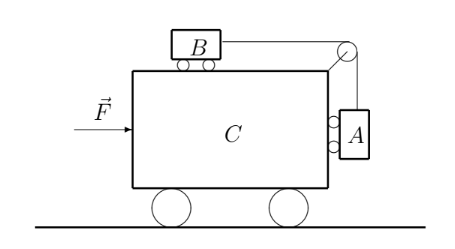
\includegraphics[scale=0.4]{./img/carrito.png}
			\caption{Ejercicio 6}
		\end{figure}
	\end{ejercicio}
	\noindent \textbf{Solución: } \\
	\begin{enumerate}[1)]
		\item Se tiene una fuerza $\vec{F}$ aplicada al carrito $C$ de tal modo que los carritos $A$ y $B$ se mantienen en reposo respecto a $C$.
		\begin{figure}[H]
			\centering
			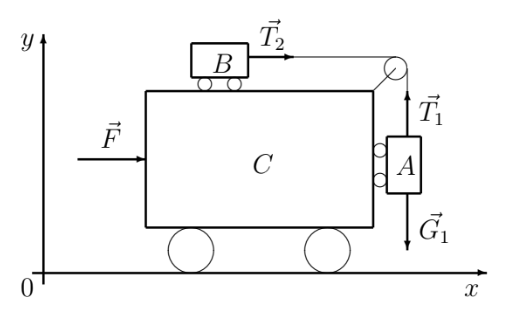
\includegraphics[scale=0.5]{./img/ej6_dcl1.png}
			\caption{DCL caso 1, ejercicio 6.}
			\label{dcl_ej6_1}
		\end{figure}
		
		\begin{enumerate}[a)]
			\item La tensión la podemos encontrar enalizando cualquiera de los bloques $A$ o $B$, sabiendo que $T_1 = T_2$
			$$ \boxed{ T = m_2 a = m_1 g. } $$
			\item La magnitud de la fuerza la podemos encontrar trabajando con el sistema en conjunto
				$$ F = (m_1 + m_2 + m_3) a, $$
			y de lo encontrado en el inciso anterior se tiene la aceleración $a = m_1 g/m_2$, entonces
				$$ \boxed{ F = (m_1 + m_2 + m_3) \frac{m_1}{m_2} g. } $$
		\end{enumerate}		
		
		\item Ahora se tiene a $C$ en reposo, y las masas $A$ y $B$ se empiezan a mover desde el reposo. 
		\begin{enumerate}[a)]
			\item La aceleración de las dos masas es la misma en magnitud, esto gracias a la "idealización" del problema. Entonces, analizando el movimiento conjunto de las dos masas, se tiene
			$$ (m_1 + m_2) a = m_1 g, $$
		despejando
			$$ \boxed{ a = \frac{m_1}{m_1 + m_2} g. } $$
			\item Para la masa $B$ se tiene la igualdad $T = m_2 a$. Reemplazando el valor encontrado de la aceleración en el inciso anterior
			$$ \boxed{ T = \frac{m_1 m_2}{m_1 + m_2} g. } $$
		\end{enumerate}	
	\end{enumerate}
\end{mdframed}





\begin{mdframed}[style=warning]
	\begin{reto}
		Un prisma triangular de masa $M$ se encuentra en un plano horizontal sin fricción. Los otros dos lados del prisma están inclinados respecto al plano unos ángulos $\alpha _1$ y $\alpha _2$ respectivamente. Dos bloques de masa $m_1$ y $m_2$, conectados por unna cuerda inelástica que pasa por una polea ideal.
	\begin{itemize}
		\item Exprese la aceleración $a$ de los bloques relativas al prisma en términos de la aceleración $a_o$ del prisma.
		\item Encuentre la aceleración $a_o$ del prisma en términos de las cantidades conocidas.
		\item ¿A qué razón $m_1 /m_2$ el prisma estará en equilibrio?
	\end{itemize}
		\begin{figure}[H]
			\centering
			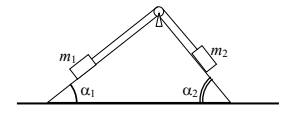
\includegraphics[scale=0.7]{./img/cunamovil.png}
			\caption{Reto.}
		\end{figure}
	\end{reto}
	\noindent \textbf{Solución: } \\
	No les compartiré solución de este problema, aún. Como les mencioné en el taller, les recomiendo intentar los problemas de \textit{"La Cuña Móvil"} y \textit{"Máquina de Atwood"} mostrados en el libro de Zemansky $13ed$. Luego de comprender esos problemas, reintenten este. Al final del semestre les compartiré la solución.
\end{mdframed}


















%%%